\documentclass[a4paper]{article}

\usepackage[slovene]{babel}
\usepackage[utf8]{inputenc}
\usepackage[T1]{fontenc}
\usepackage{lmodern}
\usepackage{amsmath}
\usepackage{amssymb}
\usepackage{amsthm}
\usepackage{amsfonts}
\usepackage{mathtools}
\usepackage{enumitem}
\usepackage[table,xcdraw]{xcolor}
\usepackage[utf8]{inputenc} 
\usepackage[T1]{fontenc}
\usepackage{graphicx}


\begin{document}

\begin{titlepage}
    \centering
    \vfill
    \vfill
    \textbf{\large{SEMINARSKA NALOGA IZ STATISTIKE - POROČILO}}
    \vfill
    \textsc{\Large{Klara Golob}}
    \vfill\vfill
    \textsc{\large{UL FMF, Matematika - univerzitetni študij}}
    
     \vfill
    \large{Avgust 2020}
    
\end{titlepage}

%%%

\newpage

%%%%%%%%%%%%%%%%%%%%%%%%%%%%%%%%%%%%%%%%%%%%%%%%%%%%%%%%%%%%%%

\large{1. NALOGA}
\\
\\
V datoteki Kibergrad se nahajajo informacije o 43.886 družinah, ki stanujejo v mestu Kibergrad. Za vsako družino so zabeleženi naslednji podatki (ne boste potrebovali vseh):
\begin{itemize}
\item Tip družine (od 1 do 3)
\item Število članov družine
\item Število otrok v družini
\item Skupni dohodek družine
\item Mestna četrt, v kateri stanuje družina (od 1 do 4)
\item Stopnja izobrazbe vodje gospodinjstva (od 31 do 46)
\end{itemize}
Nalogo sem reševala s pomočjo programskega jezika R. Zraven je priložena datotek z imenom "naloga1.R", v kateri je postopek računanja.

\begin{enumerate}[label=(\alph*)]

\item Vzemite enostavni slučajni vzorec 200 družin in na njegovi podlagi ocenite povprečno število otrok na družino v Kibergradu. 
\begin{equation*}
\hat{\mu} = \frac{1}{n} \sum_{i=1}^{n} x_{i}
\end{equation*}
Povprečno število otrok na podlagi vzorca  = $1.025$

\item Ocenite standardno napako in postavite $95\%$ interval zaupanja. \\
Varianca:
\begin{equation*}
\hat{\sigma}^2 = \frac{1}{n-1} \sum_{i=1}^{N}(\hat{\mu}-x_{i})^2
\end{equation*}
Standardna napaka:
\begin{equation*}
\widehat{ se(\hat{\sigma}}) = \sqrt{\frac{\hat{\sigma}^2}{n} \left(1-\frac{n}{N}\right) }
\end{equation*}
Standardna napaka izračunana po zgornji formuli $ = 0.07579955$ \\
Interval zaupanja $= [0.8764356, 1.173564]$

\item Vzorčno povprečje in ocenjeno standardno napako primerjajte s populacijskim povprečjem in pravo standardno napako. Ali interval zaupanja iz prejšnje točke pokrije populacijsko povprečje? \\ \\
Vzorčno povprečje = 0.92 \\
Populacijsko povprečje =  0.9479333 \\
Ocena standardne napake vzorca =  0.07579955 \\
Standardna napaka populacije =  0 \\
Razlika vzorčnega in populacijskega povprečja = 0.07706672 \\
Razlika standardnih napak = 0.07579955 \\ \\
Interval zaupanja iz prejšne točke pokrije populacijsko povprečje, saj je $0.9479333 \in [0.8764356, 1.173564]$

\item Vzemite še 99 enostavnih slučajnih vzorcev in prav tako za vsakega določite $95\%$ interval zaupanja. Narišite intervale zaupanja, ki pripadajo tem 100 vzorcem. Koliko jih pokrije populacijsko povprečje? \\ \

95 intervalov zaupanja izmed 100ih pokrije populacijsko povprečje, ker se lahko vidi tudi na sliki.

\begin{figure}[h!]
\centering
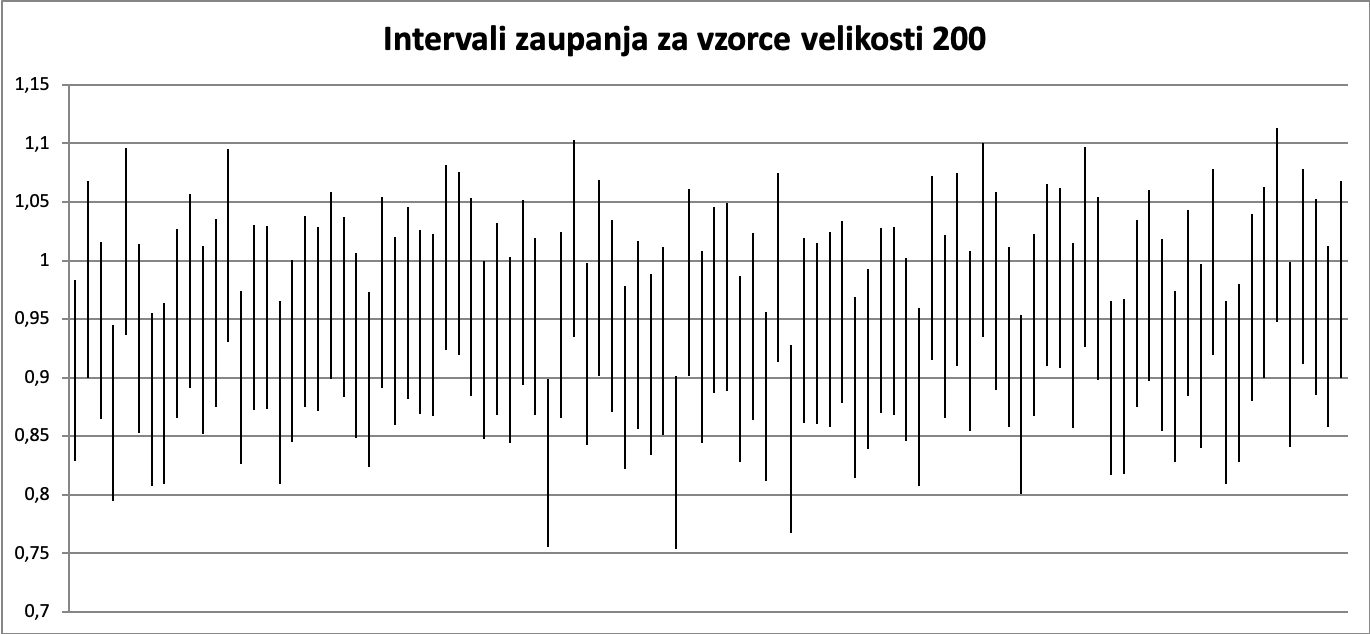
\includegraphics[width=11cm]{Intervali_zaupanja200.png}
\label{Intervali zaupanja za 100 enostavnih slučajnih vzorcev velikosti 200}
\end{figure}

\item Izračunajte standardni odklon vzorčnih povprečij za 100 prej dobljenih vzorcev. Primerjajte s pravo standardno napako za vzorec velikosti 200. \\ \\
Standardni odklon vzorčnih povprečij za 100 prej dobljenih vzorcev = 0.08253901 \\
Standardna napaka za vzorec velikosti 200 = 0.07579955 \\
Razlika = 0.006739461 

\item Izvedite prejšnji dve točki še na 100 vzorcih po 800 družin. Primerjajte in razložite razlike s teorijo vzorčenja. \\ \

96 intervalov zaupanja izmed 100ih pokrije populacijsko povprečje.
Standardni odklon vzorčnih povprečij za 100 dobljenih vzorcev veliksti 800 = 0.04111221 \\
Standardna napaka za vzorec velikosti 800 = 0.03928324 \\
Razlika = 0.001828971
Rezultati so malo bolj natančni, saj smo izbrali večji vzorec in zato dobili boljše tezultate. 
\begin{figure}[h!]
\centering
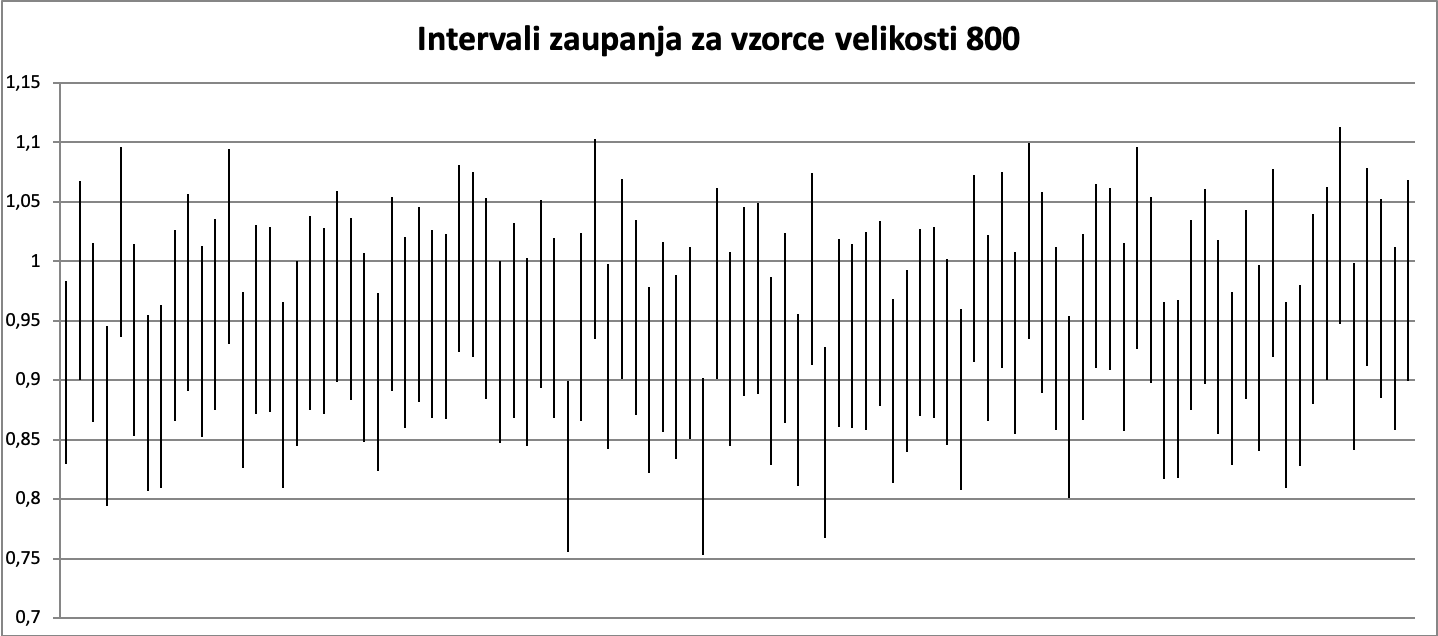
\includegraphics[width=11cm]{Intervali_zaupanja800.png}
\label{Intervali zaupanja za 100 enostavnih slučajnih vzorcev velikosti 800}
\end{figure}
\end{enumerate}

\large{2. NALOGA}
\\ \\
Populacijo sestavljajo trije stratumi, prva dva imata 1000, tretji pa ima 500 enot. Iz vsakega stratuma vzamemo enostavni slučajni vzorec desetih enot in vrednosti spremenljivke pridejo:\\ \\
1.stratum: 94 99 106 106 101 102 122 104 97 97 \\
2.stratum: 183 183 179 211 178 179 192 192 201 177 \\
3.stratum: 343 302 286 317 289 284 357 288 314 276\\ \\
Ocenite populacijsko povprečje in standardno napako vaše cenilke ter poiščite aproksimativni $95\%$ interval zaupanja. \\ \\
Velikost populacije: $N = 2500$ \\
Velikosti stratumov: $N_1 = 1000, N_2 = 1000, N_3 = 500$  \\
Velikost enostavnih slučajnih vzorcev, izbranih iz stratumov: $n_1 = n_2 = n_3 = n = 10$ \\
Velikosti deležev stratumov: $w_1 = 0.4, w_2 = 0.4, w_3 = 0.2 $ \\
Vzorčna povprečja stratumov: $\hat{\mu_1} = 98.3,  \hat{\mu_2} = 187.5,  \hat{\mu_3} = 305.6$ \\ 
\\
Ocena populacijskega povprečja:
\begin{equation*}
\hat{\mu} = w_1\hat{\mu_1} + w_2 \hat{\mu_2} + w_3 \hat{\mu_3} =  0.4 \times 98.3 + 0.4 \times 187.5 + 0.2 \times 305.6 = 175.44
\end{equation*}
Ocena kvadrata standardne napake:
 \begin{equation*}
\widehat{ se^2 }= \sum_{i=1}^{3} x_i^2 \frac{N_i-n}{N_i-1}\frac{S_i}{n_1(n_1-1)},
\end{equation*}
kjer je 
 \begin{equation*}
S_i = \sum_{j=1}^{n} (X_{ij} - \hat{\mu_i})^2 
\end{equation*}
in $X_{i1}, X_{i2} \ldots X_{in}$ vrednosti spremenljivk na enotah vzorca i-tega stratuma.

\begin{multline*}
S_1 = (94 - 98.3)^2 + (99 - 98.3)^2 + (106 - 98.3)^2 + (106 - 98.3)^2 + (101 - 98.3)^2  \\
 + (102 - 98.3)^2 + (122 - 98.3)^2 + (104 - 98.3)^2 + (97 - 98.3)^2 \\
+ (97 - 98.3)^2 = 756.1000000000001
\end{multline*}
\begin{multline*}
S_2 = (183 - 187.5)^2 + (183 - 187.5)^2 + (179 - 187.5)^2 + (211 - 187.5)^2  \\ + (178 - 187.5)^2 + (179 - 187.5)^2 + (192 - 187.5)^2 + (192 - 187.5)^2 \\ + (201 - 187.5)^2 + (177 - 187.5)^2 = 1160.5
\end{multline*}
\begin{multline*}
S_3 = (343 - 305.6)^2 + (302 - 305.6)^2 + (286 - 305.6)^2 + (317 - 305.6)^2 \\ + (289 - 305.6)^2 + (284 - 305.6)^2 + (357 - 305.6)^2 + (288 - 305.6)^2 \\ + (314 - 305.6)^2 + (276 - 305.6)^2 = 6566.400000000001
\end{multline*}
\begin{multline*}
\widehat{ se^2 }= 0.4^2 \frac{1000-10}{1000} \frac{756.1}{10(10-1)} +  0.4^2 \frac{1000-10}{1000} \frac{1160.5}{10(10-1)} + \\ 0.2^2 \frac{500-10}{500} \frac{6566.4}{10(10-1)} = 182.099
\end{multline*}
Ocena standardne napake cenilke populacijskega povprečja:
 \begin{equation*}
\hat{se}= \sqrt{\widehat{ se^2 }} = \sqrt{182.099} = 13.5
\end{equation*}
Aproksimativni $95\%$ interval zaupanja:
 \begin{equation*}
[\hat{\mu} - Z_{\alpha}\times\hat{se}, \hat{\mu} + Z_{\alpha}\times\hat{se}] = [148.98, 201.9]
\end{equation*} 

\large{3. NALOGA} \\ \\
V datoteki ZarkiGama se nahajajo podatki o časovnih razmikih med 3.935 zaznanimi fotoni, torej medprihodni časi (v sekundah).
\begin{enumerate}[label=(\alph*)]
\item Naredite histogram medprihodnih časov. Se vam zdi, da je model s porazdelitvijo gama plavzibilen?
\begin{figure}[h!]
\centering
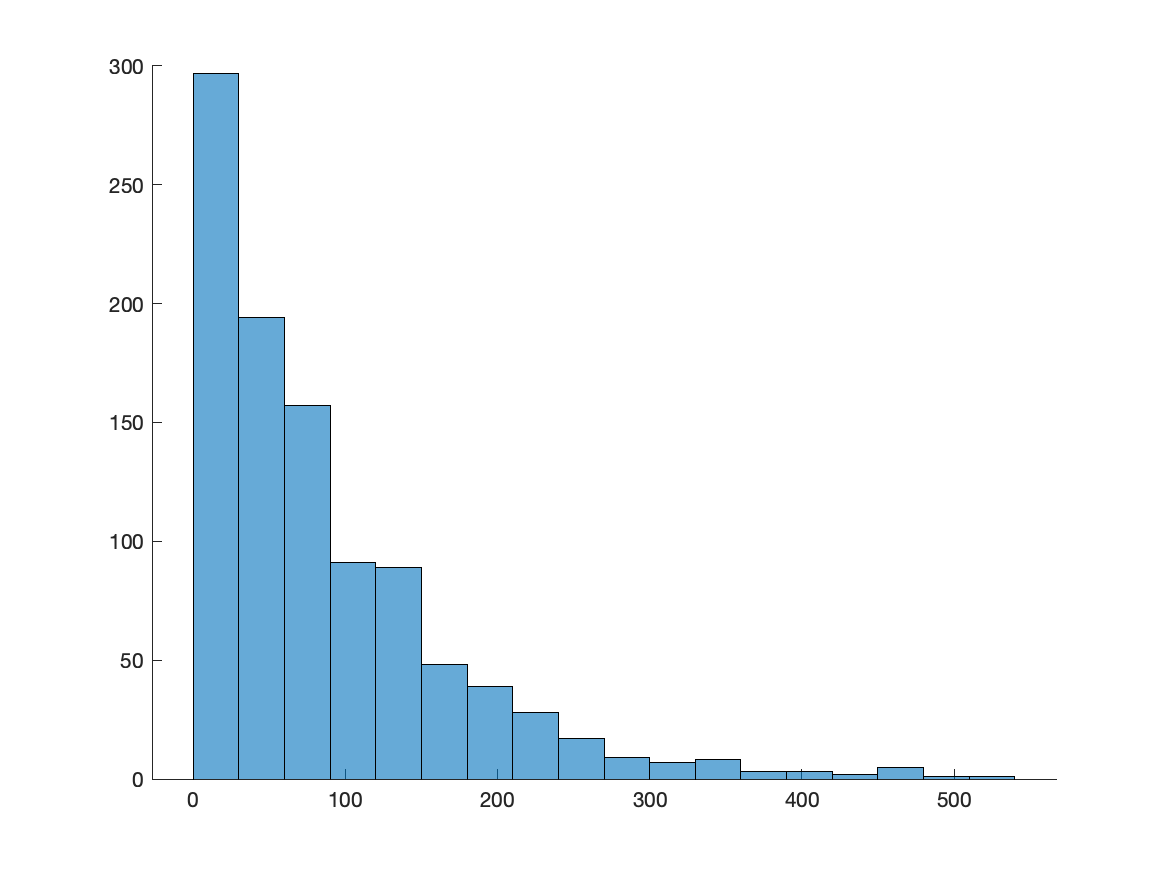
\includegraphics[width=10cm]{histogram3.png}
\label{Histogram medprehodnih časov}
\end{figure}

Glede na dobljeni histogram, je gama porazdelitev primerna.

\item Ocenite parametra porazdelitve gama po metodi momentov in po metodi največjega verjetja. Primerjajte!

$$X  \sim \Gamma(\alpha, \lambda)$$
Po metodi momentov sta cenilki za $\alpha$ in $\lambda$
$$\hat{\alpha} = \frac{\overline{X}^2}{\hat{\sigma}^2} \ \ \ \text{in} \ \ \ \hat{\lambda} = \frac{\overline{X}}{\hat{\sigma}^2} $$
$$\overline{X} = 79.93522$$
$$\hat{\sigma} = 79.45616$$
$$\hat{\alpha} = 1.0121 \ \ \  \text{in} \ \ \ \hat{\lambda} =  0.0127 $$

Po metodi najmanjših kvadratov, pa cenilki za $\alpha$ in $\lambda$ dobimo z naslednjima dvema izrazoma:
$$n\log{\hat{\alpha}} - n\log{\overline{X}} + \sum_{i=1}^{n} \log{x_i} - n\frac{\Gamma'(\hat{\alpha})}{\Gamma(\hat{\alpha})}$$
$$\hat{\lambda} = \frac{\hat{\alpha}}{\overline{X}}$$
Naj bo $F(x) = \frac{\Gamma'(x)}{\Gamma(x)}$
Potem je 
$$n\log{\hat{\alpha}} - n\log{\overline{X}} + \sum_{i=1}^{n} \log{x_i} - nF(\hat{\alpha})$$

Enačbo lahko rešimo s programom Matlab z uporabo funkcije psi in dobimo:
$$\hat{\alpha} = 1.0263 \ \ \ \text{in} \ \ \ \hat{\lambda} = 0.0128$$

\item Ocenjeni porazdelitvi dorišite na histogram. Je videti razumno?
Na grafu je z roza barvo prikazana porazdelitev po metodi momentov in z modro barvo porazdelitev po metodi največjega verjetja. Porazdelitvi ujemata med sabo in s histogramom.
\begin{figure}[h!]
\centering
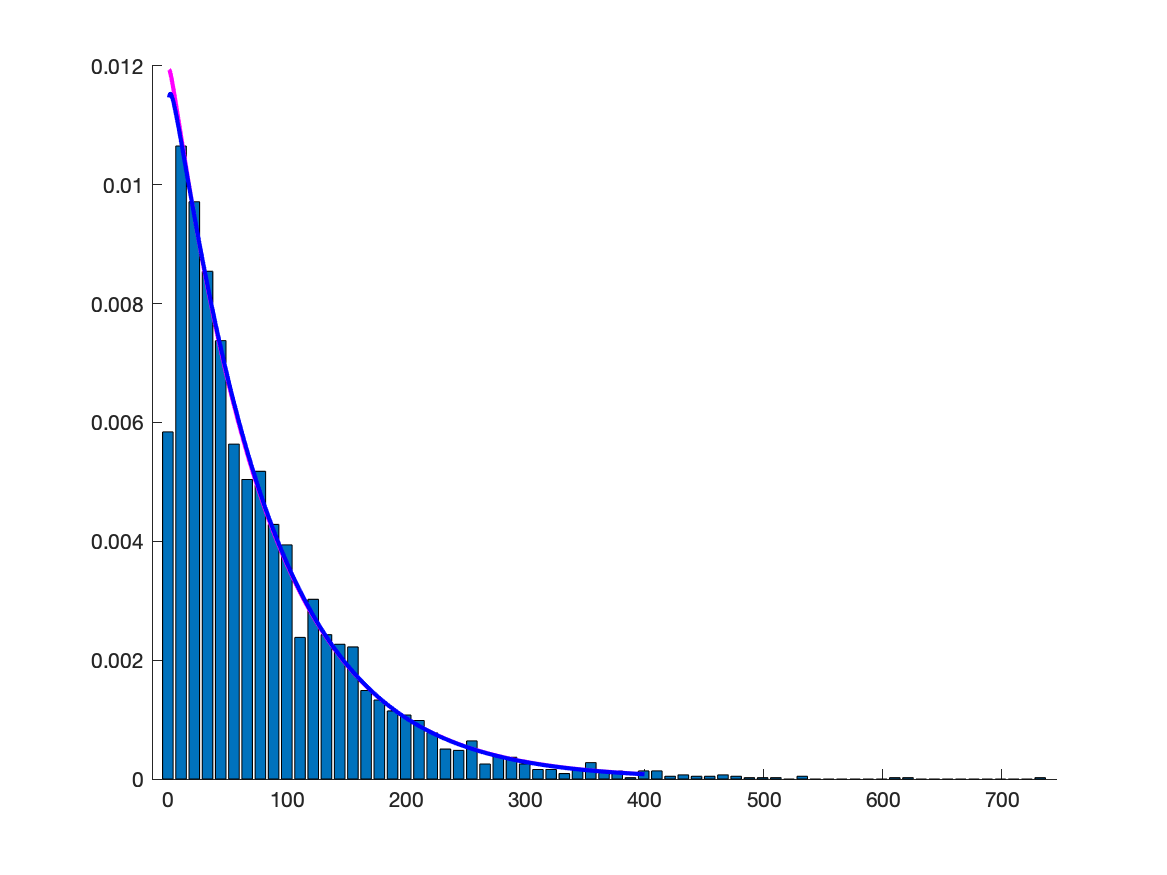
\includegraphics[width=10cm]{histogram_porazdelitve3.png}
\label{Histogram prehodnih časov z ocenjenima porazdelitvama}
\end{figure}

\item Histogram z dorisanima gostotama narišite še na logaritemski lestvici. Lestvico transformirajte le na abscisni osi, vendar pa ustrezno transformirajte tudi dorisani gostoti.

\begin{figure}[h!]
\centering
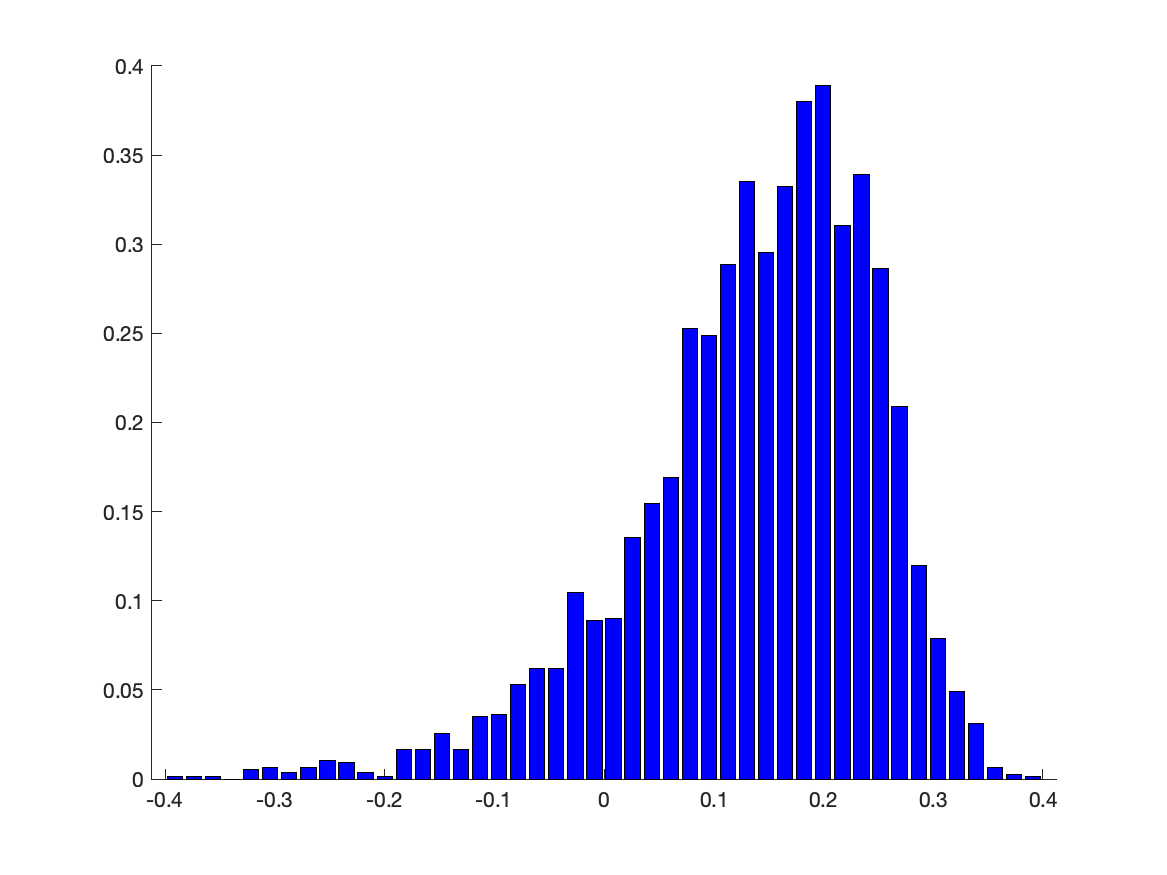
\includegraphics[width=9cm]{log_histogram3.png}
\label{Histogram prehodnih časov na logaritemski lestvici}
\end{figure}

\item Je porazdelitev medprihodnih časov videti konsistentna s Poissonovim modelom, po katerem so ti časi porazdeljeni eksponentno? \\
Da, glede na graf, bi porazdelitev medprehodnih časov lahko ustrezala tudi Poissonovi porazdelitvi. Prav tako smo prameter $\alpha$ v obeh primerih ocenili blizu 1, iz česar bi lahko rekli, da so medprehodni časi porazdeljeni Exp($\lambda$), za ustrezen $\lambda$.
\end{enumerate}

\large{4. NALOGA} \\ \\
Recimo, da opazimo eno vrednost statistične spremenljivke X, porazdeljene enakomerno na intervalu $[0, \theta]$. Preizkusimo ničelno domnevo $H_0 : \theta = 1$ proti alternativni domnevi $H_1: \theta=2$.
\begin{enumerate}[label=(\alph*)]
\item Poiščite preizkus, ki ima stopnjo tveganja $\alpha = 0$. Kolikšna je njegova moč? \\ \\
Ker je X porazdeljena enakomerno, je funkcija verjetja enaka:
$$L(\theta, x) = \frac{1}{\theta}$$


\end{enumerate}

\large{5. NALOGA} \\ \\
Naj bosta $X$ in $Y$ slučajni spremenljivki z:
    \begin{equation*} \text{E}(X) = \mu_x, \ \ \  \text{E}(Y) = \mu_y, \end{equation*}
     \begin{equation*}\text{var}(X) = \sigma_x^2 \ \ \ \text{var}(Y) = \sigma_y^2, \end{equation*}
     \begin{equation*}\text{cov}(X,Y) = \sigma_{x,y} \end{equation*}.

Denimo da opazimo $X$ in želimo napovedati $Y$.
\begin{enumerate}[label=(\alph*)]
\item Poiščite napoved oblike $Y = \alpha + \beta X$, kjer $\alpha$ in $\beta$ izberemo tako, da je srednja
kvadratična napaka $ \text{E} [ ( Y - \hat{Y} ) ^2 ]$  minimalna. Matematični upanji, varianci in kovarianco poznamo
Pomagamo si z namigom:
\begin{align*} 
    \text{E} \left[ \left( Y - \hat{Y} \right) ^2 \right] = \left[ \text{E}(Y) - \text{E}(\hat{Y}) \right]^2 + \text{var}(Y - \hat{Y}).
\end{align*}
Poiskati moramo vrednosti za $\alpha$ in $\beta$, ki minimizirata desno stran zgornje enačbe. Ker sta oba člena enkao predznačena, sta pozitivna, lahko poiščemo $\alpha$ in $\beta$, ki minimizirata vsak člen posebej. Potem bo tudi vsota teh dveh plenov minimalna. Za prvi člen velja:
\begin{equation*}
\text{E}(\hat{Y}) = \alpha + \beta \text{E}(X) =  \alpha + \beta \mu_x,
\end{equation*}
\begin{equation*}
    \left[ \text{E}(Y) - \text{E}(\hat{Y}) \right]^2 = \left[ \mu_y - \alpha - \beta \mu_x \right] ^2 .
\end{equation*}
Ta bo najmanjša, ko bo $ \mu_y - \hat{\alpha} - \beta \cdot \mu_x = 0$. Iz tega sledi:
\begin{equation*}
\hat{\alpha} = \mu_y - \beta \mu_x.
\end{equation*} 
Za drugi člen pa velja:
\begin{multline*}
\text{var}(Y-\hat{Y}) = \text{var}(Y - \alpha - \beta X) = \text{var}(Y - \beta X) = \\ \text{var}(Y) - 2 \beta \text{cov}(X, Y) + \beta^2 \text{var}(X) = \sigma_y^2 - 2 \beta \sigma_{x,y} + \beta^2 \sigma_x^2.
\end{multline*}
Minimalno vrednost izraza izračunamo tako, da izraz odvajalmo po $\beta$ in odvod izenačimo z 0.
\begin{equation*}
    \frac{\partial}{\partial \beta} (\text{var}(Y - \hat{Y})) = - 2 \sigma_{x,y} + 2 \beta \sigma_x^2 = 0 
\end{equation*}
Tako je $ \hat{\beta} = \frac{\sigma_{x,y}}{\sigma_x^2} $.
\\
Vrednosti za $\alpha$ in $\beta$, ki minimizirata $\text{E} \left[ \left( Y - \hat{Y}) \right) ^2 \right]$ sta:

$$ \hat{\alpha} = \mu_y - \mu_x \frac{\sigma_{x,y}}{\sigma_x^2} \ \ \ \ \ \text{in} \ \ \ \ \ \hat{\beta} = \frac{\sigma_{x,y}}{\sigma_x^2} $$

\item Pokažite, da se pri tako izbranih koeficientih determinacijski koeficient (kvadrat korelacijskega koeficienta) izraža v obliki:
$$ r_{x,y}^2 = 1 - \frac{\text{var}(Y - \hat{Y})}{\text{var}(Y)}. $$
Po formuli za korelacijski koeficient velja:
$$ r_{x,y}^2 = \frac{\text{cov}(X,Y)^2}{\text{var}(X) \text{var}(Y)} = 1 - \frac{\text{var}(Y - \hat{Y})}{\text{var}(Y)} = \frac{\text{var}(Y) - \text{var}(Y - \hat{Y})}{\text{var}(Y)}. $$
Iz prejšnega primera uporabimo
$$ \text{var}(Y-\hat{Y}) = \sigma_y^2 - 2 \beta \sigma_{x,y} + \beta^2 \sigma_x^2,$$
$$ \beta = \frac{\sigma_{x,y}}{\sigma_x^2}.$$
\end{enumerate}
Vstavimo v enčbo in dobimo:
\begin{multline*}
 r_{x,y}^2 = \frac{\text{var}(Y) - \text{var}(Y - \hat{Y})}{\text{var}(Y)} = \frac{\sigma_y^2 - \sigma_y^2 + \frac{\sigma_{x,y}^2}{\sigma_x^2}}{\sigma_y^2} = \frac{\sigma_{x,y}^2}{\sigma_x^2 \sigma_y^2} =\frac{\text{cov}(X,Y)^2}{\text{var}(X) \text{var}(Y)}  
\end{multline*}
S tem smo dokazali, da se res koeficientih determinacijski koeficient izraža v obliki:
$$ r_{x,y}^2 = 1 - \frac{\text{var}(Y - \hat{Y})}{\text{var}(Y)}. $$

\end{document}